\subsection{Xamarin.Android}
�hnlich wie bei Xamarin.iOS bietet Xamarin.Android die M�glichkeit native Android Apps mit Xamarin
zu erstellen. Xamarin.Android benutzt den sogenannten Just-In-Time (JIT) Compiler um eine
raffinierte Optimierung der App Performance zur Laufzeit zu erm�glichen. Eine Xamarin.Android App
ist eine native Android APK (siehe Abb. \ref{fig:abb19}). Xamarin bringt 100\% von Google�s Android API in C\#
mit.
Mit dem bereits erw�hnten automatisierten Binding-Generator lassen sich Java Code, Frameworks und
benutzerdefinierte Steuerelemente in einer Xamarin App verwenden.
\begin{figure}[!h]
\centering
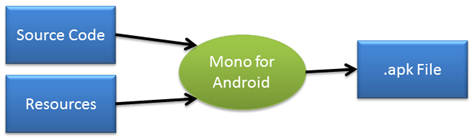
\includegraphics[scale = 0.8]{graphics/Xamarin_Android.png}
\caption{Xamarin.Android [\cite{XamAndroid}]}
\label{fig:abb19}
\end{figure} 
\\Im Gegensatz zu Xamarin.iOS kann
Xamarin.Android sowie auf Windows- als auch auf einem Mac-Rechner installiert werden. Au�er das
aktuelle Android SDK werden bei der Installation von Xamarin.Android auch alle anderen ben�tigten
Komponenten mitinstalliert. Xamarin Studio, bzw. Visual Studio stellt einen Android Emulator zur
Verf�gung, mit dem man eine App debuggen kann.

Genau wie Xamarin.iOS Entwicklung der herk�mmlichen iOS Entwicklung sehr �hnlich ist, ist auch
Xamarin.Android fast identisch mit der nativen Android App Entwicklung. Anstatt Java wird C\#
benutzt, aber die Entwicklungsans�tze sind gleich. Es werden Intents und Activities benutzt und der
Lebenszyklus einer Activity entspricht dem einer Activity aus der nativen Android App Entwicklung.
Die Ressourcen werden auch analog geordnet.
\\Gleich am Anfang, wenn ein neues Projekt erstellt wird, sollten folgende drei Einstellungen
vorgenommen werden:
\begin{itemize}
  \item Target Framework - dieses API Level wird zur Kompilierzeit benutzt und legt das Framework
  fest, mit der die App erstellt werden soll.
  \item Minimum Android Version - spezifiziert die �lteste Android Version, die die App unterst�tzen
  soll. Wird zur Laufzeit benutzt.
  \item Target Android Version - spezifiziert die Android Version auf der die App laufen soll. Wird
  zur Laufzeit benutzt.
\end{itemize}
Die verwendeten SDKs m�ssen durch den Open Android SDK Manager von Xamarin Studio (bzw. Visual
Studio) installiert werden.\\Wie bei Xamarin.iOS, bietet Xamarin.Android einen Designer f�r das
Gestalten der Benutzungsoberfl�che [\cite{XamAndroid}].